\documentclass[conference]{IEEEtran}
\IEEEoverridecommandlockouts
\usepackage{cite}
\usepackage{amsmath,amssymb,amsfonts}
\usepackage{algorithmic}
\usepackage{graphicx}
\usepackage{textcomp}
\usepackage{xcolor}
\usepackage{booktabs}
\usepackage{array}
\usepackage{url}
\usepackage{tikz}
\usetikzlibrary{arrows.meta,positioning,shapes.geometric}
\def\BibTeX{{\rm B\kern-.05em{\sc i\kern-.025em b}\kern-.08em
    T\kern-.1667em\lower.7ex\hbox{E\kern-.125emX}}}

\begin{document}

\title{MentorLink: A Verified, Analytics-Ready Platform for\ Institutional Mentorship and Impact Recognition}

% Author names intentionally left blank pending final author and affiliation details.
\author{}

\maketitle

\begin{abstract}
Institutional mentoring is commonly distributed across informal conversations, making suitable mentors difficult to discover and mentoring outcomes difficult to measure. This paper presents MentorLink, a secure web platform that formalizes institute-focused mentorship while producing structured, analytics-ready interaction data. The system combines email-verified identity, role-aware access control, mentor discovery, mentorship lifecycle management, communities, realtime collaboration, and explicit interaction confirmation. Its main contribution is a hybrid mentoring-impact model that converts confirmed sessions into auditable contribution events using activity, mentee feedback, resolved outcomes, follow-up completion, and unique mentee reach. Achievement thresholds use both quantitative and quality gates, and formal certificates are issued through SMTP and exposed in an Institute Member profile. A synthetic end-to-end evaluation of the implemented system produced 109 contribution points from three confirmed sessions involving two mentees, three resolved outcomes, three follow-ups, a 5/5 average rating, and a valid Helpful Contributor certificate. External users are restricted to seeking mentorship while retaining mentor discovery and approved community access. The implementation demonstrates how a practical mentoring platform can connect user workflows, evidence capture, explainable recognition, and privacy-aware access boundaries.
\end{abstract}

\begin{IEEEkeywords}
academic mentoring, educational technology, interaction analytics, impact scoring, achievement certificates, recommendation systems, role-based access control
\end{IEEEkeywords}

\section{Introduction}
Students frequently seek guidance about coursework, projects, placements, technical skills, and campus life. In many institutions, this guidance is exchanged through private messaging applications, personal networks, and disconnected group conversations. These channels may support communication, but they provide limited discoverability, weak accountability, and almost no structured evidence for evaluating mentoring programs.

MentorLink addresses this problem as a combined platform and data-design challenge. It provides a verified environment in which users can create academic profiles, discover potential mentors, request mentorship, communicate, participate in communities, and record mentoring interactions. The system also distinguishes between users who provide mentorship and External users who seek it. This distinction is enforced both in the interface and at the API layer.

A central design question is how a platform can recognize mentoring effort fairly. Counting requests or unverified sessions can reward activity without demonstrating useful help. MentorLink therefore introduces an auditable contribution ledger. A session becomes eligible for recognition only after the mentee confirms it. Points are then derived from multiple signals: verified activity, satisfaction, outcome resolution, follow-up completion, and the number of distinct mentees helped. Achievement certificates require minimum thresholds across these dimensions.

The contributions of this work are:
\begin{itemize}
    \item a secure, institute-oriented architecture for structured mentorship workflows;
    \item an interaction model that converts informal mentoring into analytics-ready evidence;
    \item a hybrid and explainable mentoring-impact scoring method with quality gates;
    \item a tiered achievement and certificate workflow with SMTP delivery, profile display, and public verification; and
    \item an implemented External-user boundary that preserves mentor discovery and community browsing while preventing mentor-side operations.
\end{itemize}

\section{Related Work}
Research on peer mentoring consistently identifies guidance, belonging, and social integration as important contributors to student persistence and development \cite{tinto1993,gershenfeld2014}. However, many mentoring programs still depend on manual matching and retrospective reporting. Learning analytics research emphasizes that educational systems should transform learner activity into interpretable evidence while respecting privacy and context \cite{siemens2013,ferguson2012,knox2013,drachsler2015}.

Recommendation systems provide established methods for matching users based on preferences, similarity, and behavioral evidence. Collaborative filtering and hybrid recommendation methods are useful when explicit profile information is combined with interaction history \cite{resnick1997,burke2002,ekstrand2011}. MentorLink adapts this principle to an institutional setting by combining skills, interests, academic context, availability, profile strength, and interaction analytics. Unlike a generic social recommender, the system also applies eligibility constraints such as academic progression and mentor consent.

Recognition systems introduce a second design problem. A purely volume-based score is easy to explain but vulnerable to repetitive or low-value activity. A purely outcome-based score may be difficult to measure and may unfairly penalize mentors working on longer-term goals. MentorLink therefore uses a transparent hybrid model: auditable events provide the point total, while minimum session, reach, outcome, and rating requirements prevent a certificate from being earned through volume alone.

\section{System Requirements and Design Goals}
The system was designed around five requirements. First, only verified users should access protected platform operations. Second, mentorship should be represented as a lifecycle rather than a single message: request, acceptance, interaction, confirmation, and outcome. Third, stored interaction data should support aggregation and future recommendation experiments. Fourth, recognition should be understandable to users and traceable to evidence. Fifth, External users should have a constrained seeking-oriented experience that does not expose mentor or administrative operations.

The design goals are therefore security, explainability, modularity, privacy-aware visibility, and low operational complexity. The active application uses static browser pages backed by an Express API. MongoDB and Mongoose store semi-structured profiles, relationships, interactions, contribution events, achievements, and certificates. Socket.IO supplies realtime presence, rooms, typing events, and notifications, while REST endpoints remain the source of truth for persisted records.

\section{Architecture}
Figure~\ref{fig:architecture} summarizes the deployed architecture.

\begin{figure*}[t]
\centering
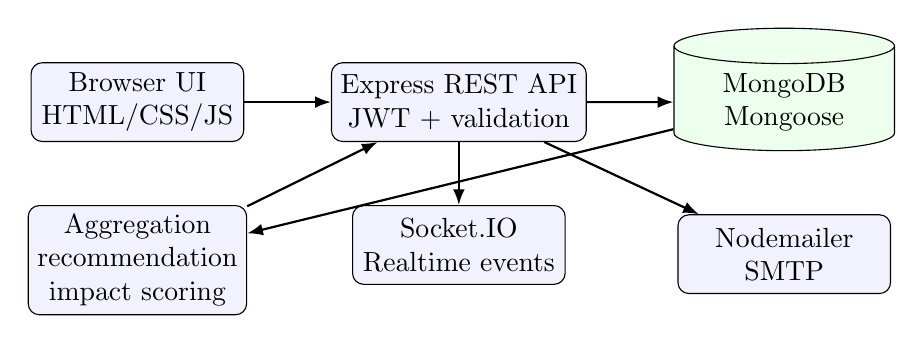
\begin{tikzpicture}[
  node distance=8mm and 11mm,
  box/.style={draw, rounded corners, align=center, minimum height=10mm, minimum width=27mm, fill=blue!5},
  store/.style={draw, cylinder, shape border rotate=90, aspect=0.25, align=center, minimum height=13mm, minimum width=28mm, fill=green!7},
  arrow/.style={-{Latex[length=2mm]}, thick}
]
\node[box] (browser) {Browser UI\\HTML/CSS/JS};
\node[box, right=of browser] (api) {Express REST API\\JWT + validation};
\node[store, right=of api] (db) {MongoDB\\Mongoose};
\node[box, below=of api] (socket) {Socket.IO\\Realtime events};
\node[box, below=of db] (email) {Nodemailer\\SMTP};
\node[box, below=of browser] (analytics) {Aggregation\\recommendation\\impact scoring};
\draw[arrow] (browser) -- (api);
\draw[arrow] (api) -- (db);
\draw[arrow] (api) -- (socket);
\draw[arrow] (api) -- (email);
\draw[arrow] (db) -- (analytics);
\draw[arrow] (analytics) -- (api);
\end{tikzpicture}
\caption{MentorLink architecture and evidence flow.}
\label{fig:architecture}
\end{figure*}

The server loads environment configuration, initializes security middleware, connects to MongoDB before listening, mounts feature routers, serves uploaded assets, and serves the static public application. The principal route groups are authentication, users, mentorships, interactions, communities, groups, chat, notifications, recommendations, and achievements.

Authentication uses email OTP verification, bcrypt password hashing, and signed JWTs. Protected requests carry a Bearer token. Middleware resolves the authenticated user and checks that the account is active. Request validation is implemented with express-validator, while rate limiting and security headers are applied at the application and route levels.

\section{Mentorship and Interaction Methodology}
A User document stores identity, account type, role, academic context, skills, interests, availability, mentorship intent, and profile information. A Mentorship document stores requester and recipient relationships, status, reasons, timestamps, and the private chat group created after acceptance.

The Interaction schema is the primary analytics entity. It includes mentor and mentee references, mentorship reference, topic, subject tag, interaction type, duration, satisfaction rating, outcome status, mentee recommendation, follow-up completion, notes, timestamp, and confirmation state. Indexes support queries by participant, mentorship, subject, type, status, and time.

A session is initially marked \texttt{pending}. The mentee confirms the session through \texttt{POST /api/interactions/:id/confirm}. The confirmation route verifies that the actor is the mentee, marks the interaction as confirmed, and invokes the contribution service. This prevents an unconfirmed mentor-created record from immediately producing recognition.

\section{Hybrid Impact Scoring}
The scoring method is deliberately transparent. For each confirmed interaction, the service creates idempotent contribution events. The event types and point ranges are shown in Table~\ref{tab:events}.

\begin{table}[t]
\caption{Contribution event model}
\label{tab:events}
\centering
\begin{tabular}{p{0.47\columnwidth}r}
\toprule
Evidence event & Points \\
\midrule
Verified activity with duration cap & 6--10 \\
Satisfaction rating & 0--10 \\
Resolved mentoring outcome & 10 \\
Completed follow-up & 5 \\
First confirmed interaction with a mentee & 5 \\
\bottomrule
\end{tabular}
\end{table}

For a mentor $m$, the contribution total is the sum of auditable event points:
\begin{equation}
P_m = \sum_{e \in E_m} p(e),
\end{equation}
where $E_m$ is the set of contribution events tied to confirmed interactions for $m$. Eligibility is not determined by $P_m$ alone. A level $l$ is awarded only if:
\begin{equation}
P_m \geq T_l,\quad I_m \geq I_l,\quad U_m \geq U_l,
\end{equation}
\begin{equation}
R_m \geq R_l,\quad \bar{S}_m \geq S_l,
\end{equation}
where $I_m$ is confirmed interactions, $U_m$ is unique mentees, $R_m$ is resolved outcomes, and $\bar{S}_m$ is average satisfaction.

The five implemented levels are Helpful Contributor, Peer Mentor, Trusted Mentor, Mentor Champion, and Mentor Excellence Award. Thresholds range from 50 to 1000 points, with increasing requirements for sessions, unique mentees, resolved outcomes, and average rating. Since events use a unique interaction-event index and are inserted with upsert semantics, retrying confirmation does not duplicate points.

\section{Certificate Issuance and User Experience}
When the highest newly eligible achievement is detected, an Achievement record is created once for the mentor and level. A Certificate record stores the certificate identifier, recipient, achievement, point total, confirmed sessions, mentees helped, average rating, issue date, and revocation state.

The certificate workflow has three delivery surfaces. First, the configured SMTP service receives an email notification when a new certificate is created. The email includes the achievement summary and a formal certificate HTML attachment. Second, Institute Member profiles contain a separate Mentor Achievements section. Third, the Achievements page displays all predefined levels: earned levels expose a \textit{View certificate} action, while locked levels show their remaining requirements.

The certificate view is a formal printable document rather than a plain data page. It contains MentorLink branding, a double border, a certificate heading, recipient name, achievement distinction, evidence metrics, certificate ID, issue date, and a verification link. Public verification returns a limited safe response with recipient name, title, issue date, certificate ID, and validity state.

\section{External-User Boundary}
External users are seeking-only participants. Their interface keeps Feed, Media, mentor discovery, outgoing requests, and community browsing and membership. External users cannot access Messages, groups, private mentorship chat, Achievements, personal certificate data, mentor interaction logging, incoming request management, community creation, or moderation. Public certificate verification remains available so an issued certificate can be independently validated.

The boundary is enforced in two layers. The browser hides unavailable navigation and profile sections, labels External profiles, and removes mentor-intent choices. The API rejects unauthorized operations even when a client bypasses the UI. For example, External requests to \texttt{/api/achievements/me}, \texttt{/api/groups}, and group chat endpoints return HTTP 403, while approved community browsing remains available.

\section{Implementation Evaluation}
The implementation was evaluated through source diagnostics, module loading, MongoDB-backed simulation, browser checks, and endpoint checks. A synthetic test account was used to avoid claiming that the measured values were collected from a production population.

For the verified Chetan test account, the system produced 109 contribution points, 3 confirmed sessions, 2 unique mentees, 3 resolved outcomes, 3 completed follow-ups, a 5/5 average rating, and a 100\% recommendation rate. The system issued a Helpful Contributor certificate with identifier \texttt{ML-2026-EA853FAE}. The certificate was retrieved through the authenticated achievements endpoint, rendered in the profile, viewed as a formal certificate, downloaded as HTML, and verified publicly.

\begin{table}[t]
\caption{End-to-end role-based endpoint checks}
\label{tab:checks}
\centering
\begin{tabular}{p{0.62\columnwidth}c}
\toprule
Check & HTTP result \\
\midrule
Institute Member authentication & 200 \\
Institute Member achievements & 200 \\
Certificate verification & 200 \\
External achievements & 403 \\
External standalone groups & 403 \\
External group chat & 403 \\
External community browsing & 200 \\
\bottomrule
\end{tabular}
\end{table}

The results demonstrate functional consistency across database records, API responses, and browser views. They do not constitute a population-level causal measurement of mentoring effectiveness. The synthetic evaluation validates the implementation path and the evidence-to-certificate contract.

\section{Security, Privacy, and Limitations}
The platform applies JWT authentication, bcrypt password hashing, OTP verification, validation middleware, security headers, rate limiting, role checks, restricted uploads, and request-time community visibility, following common web application security priorities \cite{owasp2021}. Certificate verification exposes only information intended for public validation. Admission information is treated as private profile data.

Several limitations remain. The pending registration map is process-local and should be replaced with a durable store such as Redis or a pending-user collection for production. The root automated test command is not yet a full test suite. Certificate revocation and administrative audit controls are not yet exposed as a complete management UI. The scoring model is interpretable but its weights require longitudinal validation with real mentoring outcomes. SMTP acceptance was tested through Nodemailer; actual mailbox receipt depends on the configured provider and account.

\section{Conclusion and Future Work}
MentorLink demonstrates an implementable approach for turning informal institutional mentoring into a verified, analytics-ready workflow. The system combines secure identity, constrained user roles, mentorship lifecycle management, explicit interaction confirmation, hybrid contribution scoring, and tiered certificate recognition. The design avoids equating activity volume with impact by requiring evidence from feedback, outcomes, follow-up, and mentee reach.

Future work includes durable pending-registration storage, automated integration tests, certificate administration and revocation, longitudinal validation of impact weights, richer outcome instruments, and privacy-preserving institutional analytics. With these extensions, MentorLink can evolve from a functional platform prototype into a measurable support infrastructure for academic mentoring programs.

\bibliographystyle{IEEEtran}
\bibliography{bibliography}

\end{document}
